\documentclass[twoside]{book}

% Packages required by doxygen
\usepackage{fixltx2e}
\usepackage{calc}
\usepackage{doxygen}
\usepackage[export]{adjustbox} % also loads graphicx
\usepackage{graphicx}
\usepackage[utf8]{inputenc}
\usepackage{makeidx}
\usepackage{multicol}
\usepackage{multirow}
\PassOptionsToPackage{warn}{textcomp}
\usepackage{textcomp}
\usepackage[nointegrals]{wasysym}
\usepackage[table]{xcolor}

% NLS support packages
\usepackage[T2A]{fontenc}
\usepackage[ukrainian]{babel}

% Font selection
\usepackage[T1]{fontenc}
\usepackage[scaled=.90]{helvet}
\usepackage{courier}
\usepackage{amssymb}
\usepackage{sectsty}
\renewcommand{\familydefault}{\sfdefault}
\allsectionsfont{%
  \fontseries{bc}\selectfont%
  \color{darkgray}%
}
\renewcommand{\DoxyLabelFont}{%
  \fontseries{bc}\selectfont%
  \color{darkgray}%
}
\newcommand{\+}{\discretionary{\mbox{\scriptsize$\hookleftarrow$}}{}{}}

% Page & text layout
\usepackage{geometry}
\geometry{%
  a4paper,%
  top=2.5cm,%
  bottom=2.5cm,%
  left=2.5cm,%
  right=2.5cm%
}
\tolerance=750
\hfuzz=15pt
\hbadness=750
\setlength{\emergencystretch}{15pt}
\setlength{\parindent}{0cm}
\setlength{\parskip}{3ex plus 2ex minus 2ex}
\makeatletter
\renewcommand{\paragraph}{%
  \@startsection{paragraph}{4}{0ex}{-1.0ex}{1.0ex}{%
    \normalfont\normalsize\bfseries\SS@parafont%
  }%
}
\renewcommand{\subparagraph}{%
  \@startsection{subparagraph}{5}{0ex}{-1.0ex}{1.0ex}{%
    \normalfont\normalsize\bfseries\SS@subparafont%
  }%
}
\makeatother

% Headers & footers
\usepackage{fancyhdr}
\pagestyle{fancyplain}
\fancyhead[LE]{\fancyplain{}{\bfseries\thepage}}
\fancyhead[CE]{\fancyplain{}{}}
\fancyhead[RE]{\fancyplain{}{\bfseries\leftmark}}
\fancyhead[LO]{\fancyplain{}{\bfseries\rightmark}}
\fancyhead[CO]{\fancyplain{}{}}
\fancyhead[RO]{\fancyplain{}{\bfseries\thepage}}
\fancyfoot[LE]{\fancyplain{}{}}
\fancyfoot[CE]{\fancyplain{}{}}
\fancyfoot[RE]{\fancyplain{}{\bfseries\scriptsize Створено системою Doxygen }}
\fancyfoot[LO]{\fancyplain{}{\bfseries\scriptsize Створено системою Doxygen }}
\fancyfoot[CO]{\fancyplain{}{}}
\fancyfoot[RO]{\fancyplain{}{}}
\renewcommand{\footrulewidth}{0.4pt}
\renewcommand{\chaptermark}[1]{%
  \markboth{#1}{}%
}
\renewcommand{\sectionmark}[1]{%
  \markright{\thesection\ #1}%
}

% Indices & bibliography
\usepackage{natbib}
\usepackage[titles]{tocloft}
\setcounter{tocdepth}{3}
\setcounter{secnumdepth}{5}
\makeindex

% Hyperlinks (required, but should be loaded last)
\usepackage{ifpdf}
\ifpdf
  \usepackage[pdftex,pagebackref=true]{hyperref}
\else
  \usepackage[ps2pdf,pagebackref=true]{hyperref}
\fi
\hypersetup{%
  colorlinks=true,%
  linkcolor=blue,%
  citecolor=blue,%
  unicode%
}

% Custom commands
\newcommand{\clearemptydoublepage}{%
  \newpage{\pagestyle{empty}\cleardoublepage}%
}

\usepackage{caption}
\captionsetup{labelsep=space,justification=centering,font={bf},singlelinecheck=off,skip=4pt,position=top}

%===== C O N T E N T S =====

\begin{document}

% Titlepage & ToC
\hypersetup{pageanchor=false,
             bookmarksnumbered=true,
             pdfencoding=unicode
            }
\pagenumbering{roman}
\begin{titlepage}
\vspace*{7cm}
\begin{center}%
{\Large My Project }\\
\vspace*{1cm}
{\large Створено системою Doxygen 1.8.11}\\
\end{center}
\end{titlepage}
\clearemptydoublepage
\tableofcontents
\clearemptydoublepage
\pagenumbering{arabic}
\hypersetup{pageanchor=true}

%--- Begin generated contents ---
\chapter{Список завдань}
\label{todo}
\hypertarget{todo}{}

\begin{DoxyRefList}
\item[\label{todo__todo000001}%
\hypertarget{todo__todo000001}{}%
Елемент \hyperlink{class_tests_1_1_form1_a861240fc111a9f0c68cdc64138e1a8e3}{Tests.Form1.button\+\_\+\+Sign\+In\+\_\+\+Click} (object sender, Event\+Args e)]something 
\end{DoxyRefList}
\chapter{Алфавітний покажчик простору імен}
\section{Пакети}
Повний список документованих пакетів.\begin{DoxyCompactList}
\item\contentsline{section}{\hyperlink{namespace_tests}{Tests} }{\pageref{namespace_tests}}{}
\end{DoxyCompactList}

\chapter{Ієрархічний покажчик класів}
\section{Ієрархія класів}
Список успадкувань впорядковано наближено до алфавіту\begin{DoxyCompactList}
\item Form\begin{DoxyCompactList}
\item \contentsline{section}{Tests.\+Adminka}{\pageref{class_tests_1_1_adminka}}{}
\item \contentsline{section}{Tests.\+Form1}{\pageref{class_tests_1_1_form1}}{}
\item \contentsline{section}{Tests.\+Form2}{\pageref{class_tests_1_1_form2}}{}
\end{DoxyCompactList}
\item \contentsline{section}{Tests.\+Program}{\pageref{class_tests_1_1_program}}{}
\end{DoxyCompactList}

\chapter{Алфавітний покажчик класів}
\section{Класи}
Класи, структури, об\textquotesingle{}єднання та інтерфейси з коротким описом.\begin{DoxyCompactList}
\item\contentsline{section}{\hyperlink{class_tests_1_1_adminka}{Tests.\+Adminka} }{\pageref{class_tests_1_1_adminka}}{}
\item\contentsline{section}{\hyperlink{class_tests_1_1_form1}{Tests.\+Form1} }{\pageref{class_tests_1_1_form1}}{}
\item\contentsline{section}{\hyperlink{class_tests_1_1_form2}{Tests.\+Form2} }{\pageref{class_tests_1_1_form2}}{}
\item\contentsline{section}{\hyperlink{class_tests_1_1_program}{Tests.\+Program} }{\pageref{class_tests_1_1_program}}{}
\end{DoxyCompactList}

\chapter{Покажчик файлв}
\section{Файли}
Повний список файлів.\begin{DoxyCompactList}
\item\contentsline{section}{\hyperlink{_adminka_8cs}{Adminka.\+cs} }{\pageref{_adminka_8cs}}{}
\item\contentsline{section}{\hyperlink{_adminka_8_designer_8cs}{Adminka.\+Designer.\+cs} }{\pageref{_adminka_8_designer_8cs}}{}
\item\contentsline{section}{\hyperlink{_form1_8cs}{Form1.\+cs} }{\pageref{_form1_8cs}}{}
\item\contentsline{section}{\hyperlink{_form1_8_designer_8cs}{Form1.\+Designer.\+cs} }{\pageref{_form1_8_designer_8cs}}{}
\item\contentsline{section}{\hyperlink{_form2_8cs}{Form2.\+cs} }{\pageref{_form2_8cs}}{}
\item\contentsline{section}{\hyperlink{_form2_8_designer_8cs}{Form2.\+Designer.\+cs} }{\pageref{_form2_8_designer_8cs}}{}
\item\contentsline{section}{\hyperlink{_program_8cs}{Program.\+cs} }{\pageref{_program_8cs}}{}
\end{DoxyCompactList}

\chapter{Опис простору імен}
\hypertarget{namespace_tests}{}\section{Простір імен Tests}
\label{namespace_tests}\index{Tests@{Tests}}
\subsection*{Класи}
\begin{DoxyCompactItemize}
\item 
class \hyperlink{class_tests_1_1_adminka}{Adminka}
\item 
class \hyperlink{class_tests_1_1_form1}{Form1}
\item 
class \hyperlink{class_tests_1_1_form2}{Form2}
\item 
class \hyperlink{class_tests_1_1_program}{Program}
\end{DoxyCompactItemize}

\chapter{Класи}
\hypertarget{class_tests_1_1_adminka}{}\section{Клас Tests.\+Adminka}
\label{class_tests_1_1_adminka}\index{Tests.\+Adminka@{Tests.\+Adminka}}
Схема успадкувань для Tests.\+Adminka\begin{figure}[H]
\begin{center}
\leavevmode
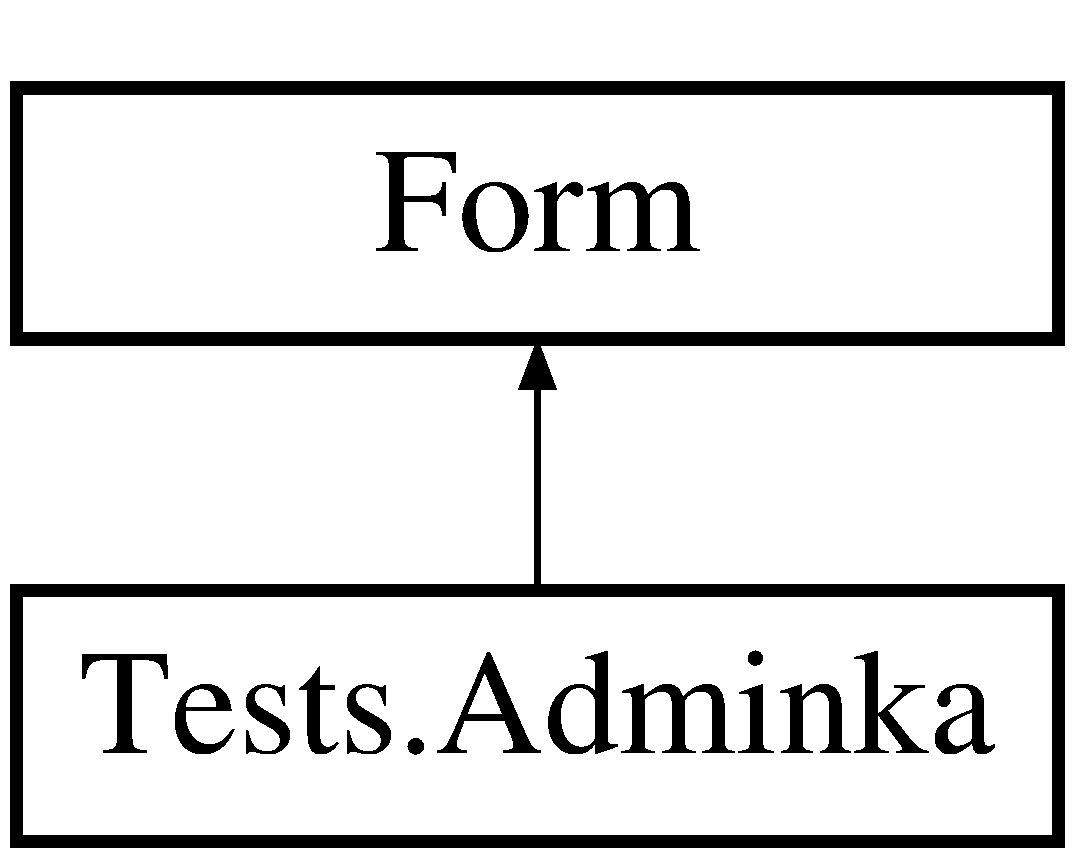
\includegraphics[height=2.000000cm]{class_tests_1_1_adminka}
\end{center}
\end{figure}
\subsection*{Загальнодоступні елементи}
\begin{DoxyCompactItemize}
\item 
\hyperlink{class_tests_1_1_adminka_afe133ffb1d1a8906368ca768606e6b72}{Adminka} ()
\end{DoxyCompactItemize}
\subsection*{Захищені елементи}
\begin{DoxyCompactItemize}
\item 
override void \hyperlink{class_tests_1_1_adminka_ad10de447810a69558e83dcdb58681510}{Dispose} (bool disposing)
\begin{DoxyCompactList}\small\item\em Clean up any resources being used. \end{DoxyCompactList}\end{DoxyCompactItemize}
\subsection*{Приватні елементи}
\begin{DoxyCompactItemize}
\item 
void \hyperlink{class_tests_1_1_adminka_a4201ca9bd4ac62e04d9c78dea1d28d6a}{button\+\_\+create\+Tema\+\_\+\+Click} (object sender, Event\+Args e)
\item 
void \hyperlink{class_tests_1_1_adminka_a74fd18bdc1977e716dbbfd8731d4bac4}{button\+\_\+\+Add\+Question\+Answer\+\_\+\+Click} (object sender, Event\+Args e)
\item 
void \hyperlink{class_tests_1_1_adminka_a997dd067679209e51d7388b408a9b8e8}{button\+\_\+save\+Tema\+\_\+\+Click} (object sender, Event\+Args e)
\item 
void \hyperlink{class_tests_1_1_adminka_a68c3719cadde4c89a1c3c949de576e9a}{button\+\_\+delete\+Question\+\_\+\+Click} (object sender, Event\+Args e)
\item 
void \hyperlink{class_tests_1_1_adminka_a717ad362ec305b9b4d9781dc509b9d3b}{Initialize\+Component} ()
\begin{DoxyCompactList}\small\item\em Required method for Designer support -\/ do not modify the contents of this method with the code editor. \end{DoxyCompactList}\end{DoxyCompactItemize}
\subsection*{Приватні дані}
\begin{DoxyCompactItemize}
\item 
List$<$ string $>$ \hyperlink{class_tests_1_1_adminka_a330050adb0204a625889fb83a3076020}{st} = new List$<$string$>$()
\item 
string \hyperlink{class_tests_1_1_adminka_aee4c653fce4f868e0443f71f103073f5}{path} = null
\item 
System.\+Component\+Model.\+I\+Container \hyperlink{class_tests_1_1_adminka_aa90b2e5b943bff4a2d5f567cd0440ace}{components} = null
\begin{DoxyCompactList}\small\item\em Required designer variable. \end{DoxyCompactList}\item 
System.\+Windows.\+Forms.\+Text\+Box \hyperlink{class_tests_1_1_adminka_ae9d52a9b2893c5ea478b87306fb97bb5}{text\+Box\+\_\+\+Question}
\item 
System.\+Windows.\+Forms.\+Text\+Box \hyperlink{class_tests_1_1_adminka_afff68b1022251085154e49d62a23384c}{text\+Box\+\_\+answer2}
\item 
System.\+Windows.\+Forms.\+Text\+Box \hyperlink{class_tests_1_1_adminka_ae3b9da7c9adc45d124cd949d7e36fa49}{text\+Box\+\_\+answer3}
\item 
System.\+Windows.\+Forms.\+Text\+Box \hyperlink{class_tests_1_1_adminka_a6ddfc84b04cb9ee0da0d214993156a13}{text\+Box\+\_\+answer1}
\item 
System.\+Windows.\+Forms.\+Label \hyperlink{class_tests_1_1_adminka_a79972d46b6074e3267bc67a0ebb2b469}{label1}
\item 
System.\+Windows.\+Forms.\+Label \hyperlink{class_tests_1_1_adminka_a4e29fe60d58caf22ebd38a346fe0642b}{label2}
\item 
System.\+Windows.\+Forms.\+Label \hyperlink{class_tests_1_1_adminka_a1fd7ef809e9adab2568fd45e3b2c2206}{label3}
\item 
System.\+Windows.\+Forms.\+Label \hyperlink{class_tests_1_1_adminka_a6d79a07b77f8747b51fc2fdae76cd37e}{label4}
\item 
System.\+Windows.\+Forms.\+List\+Box \hyperlink{class_tests_1_1_adminka_a2fdae13c03c82b36031341dd4990803f}{list\+Box\+\_\+\+Question}
\item 
System.\+Windows.\+Forms.\+Text\+Box \hyperlink{class_tests_1_1_adminka_a8636ea15196a859ed3d64c6f32ea5afc}{text\+Box\+\_\+tema}
\item 
System.\+Windows.\+Forms.\+Label \hyperlink{class_tests_1_1_adminka_ad8ff4a93c8081fe3b0bf11d4dc72e07f}{label\+\_\+tema}
\item 
System.\+Windows.\+Forms.\+Button \hyperlink{class_tests_1_1_adminka_a0e4ec04e750e175c7d5704e1332dceae}{button\+\_\+create\+Tema}
\item 
System.\+Windows.\+Forms.\+Radio\+Button \hyperlink{class_tests_1_1_adminka_abc6ff687eb6405c378c69eb77c0a531c}{radio\+Button1}
\item 
System.\+Windows.\+Forms.\+Radio\+Button \hyperlink{class_tests_1_1_adminka_aa749fca4eac152a213b3e82e9e530374}{radio\+Button2}
\item 
System.\+Windows.\+Forms.\+Radio\+Button \hyperlink{class_tests_1_1_adminka_a9c6475158496e79903d5f8b432b697a4}{radio\+Button3}
\item 
System.\+Windows.\+Forms.\+Button \hyperlink{class_tests_1_1_adminka_a4bc4d7b76649970aecb3ec1c0134db3e}{button\+\_\+save\+Tema}
\item 
System.\+Windows.\+Forms.\+Button \hyperlink{class_tests_1_1_adminka_a7606d35c26138dcc8bdc82b124fc5127}{button\+\_\+delete\+Question}
\item 
System.\+Windows.\+Forms.\+Button \hyperlink{class_tests_1_1_adminka_a3f3c6955ab04801a545f03e4045c0f19}{button\+\_\+\+Add\+Question\+Answer}
\end{DoxyCompactItemize}


\subsection{Конструктор(и)}
\index{Tests\+::\+Adminka@{Tests\+::\+Adminka}!Adminka@{Adminka}}
\index{Adminka@{Adminka}!Tests\+::\+Adminka@{Tests\+::\+Adminka}}
\subsubsection[{\texorpdfstring{Adminka()}{Adminka()}}]{\setlength{\rightskip}{0pt plus 5cm}Tests.\+Adminka.\+Adminka (
\begin{DoxyParamCaption}
{}
\end{DoxyParamCaption}
)}\hypertarget{class_tests_1_1_adminka_afe133ffb1d1a8906368ca768606e6b72}{}\label{class_tests_1_1_adminka_afe133ffb1d1a8906368ca768606e6b72}


\subsection{Опис методів компонент}
\index{Tests\+::\+Adminka@{Tests\+::\+Adminka}!button\+\_\+\+Add\+Question\+Answer\+\_\+\+Click@{button\+\_\+\+Add\+Question\+Answer\+\_\+\+Click}}
\index{button\+\_\+\+Add\+Question\+Answer\+\_\+\+Click@{button\+\_\+\+Add\+Question\+Answer\+\_\+\+Click}!Tests\+::\+Adminka@{Tests\+::\+Adminka}}
\subsubsection[{\texorpdfstring{button\+\_\+\+Add\+Question\+Answer\+\_\+\+Click(object sender, Event\+Args e)}{button_AddQuestionAnswer_Click(object sender, EventArgs e)}}]{\setlength{\rightskip}{0pt plus 5cm}void Tests.\+Adminka.\+button\+\_\+\+Add\+Question\+Answer\+\_\+\+Click (
\begin{DoxyParamCaption}
\item[{object}]{sender, }
\item[{Event\+Args}]{e}
\end{DoxyParamCaption}
)\hspace{0.3cm}{\ttfamily [private]}}\hypertarget{class_tests_1_1_adminka_a74fd18bdc1977e716dbbfd8731d4bac4}{}\label{class_tests_1_1_adminka_a74fd18bdc1977e716dbbfd8731d4bac4}
\index{Tests\+::\+Adminka@{Tests\+::\+Adminka}!button\+\_\+create\+Tema\+\_\+\+Click@{button\+\_\+create\+Tema\+\_\+\+Click}}
\index{button\+\_\+create\+Tema\+\_\+\+Click@{button\+\_\+create\+Tema\+\_\+\+Click}!Tests\+::\+Adminka@{Tests\+::\+Adminka}}
\subsubsection[{\texorpdfstring{button\+\_\+create\+Tema\+\_\+\+Click(object sender, Event\+Args e)}{button_createTema_Click(object sender, EventArgs e)}}]{\setlength{\rightskip}{0pt plus 5cm}void Tests.\+Adminka.\+button\+\_\+create\+Tema\+\_\+\+Click (
\begin{DoxyParamCaption}
\item[{object}]{sender, }
\item[{Event\+Args}]{e}
\end{DoxyParamCaption}
)\hspace{0.3cm}{\ttfamily [private]}}\hypertarget{class_tests_1_1_adminka_a4201ca9bd4ac62e04d9c78dea1d28d6a}{}\label{class_tests_1_1_adminka_a4201ca9bd4ac62e04d9c78dea1d28d6a}
\index{Tests\+::\+Adminka@{Tests\+::\+Adminka}!button\+\_\+delete\+Question\+\_\+\+Click@{button\+\_\+delete\+Question\+\_\+\+Click}}
\index{button\+\_\+delete\+Question\+\_\+\+Click@{button\+\_\+delete\+Question\+\_\+\+Click}!Tests\+::\+Adminka@{Tests\+::\+Adminka}}
\subsubsection[{\texorpdfstring{button\+\_\+delete\+Question\+\_\+\+Click(object sender, Event\+Args e)}{button_deleteQuestion_Click(object sender, EventArgs e)}}]{\setlength{\rightskip}{0pt plus 5cm}void Tests.\+Adminka.\+button\+\_\+delete\+Question\+\_\+\+Click (
\begin{DoxyParamCaption}
\item[{object}]{sender, }
\item[{Event\+Args}]{e}
\end{DoxyParamCaption}
)\hspace{0.3cm}{\ttfamily [private]}}\hypertarget{class_tests_1_1_adminka_a68c3719cadde4c89a1c3c949de576e9a}{}\label{class_tests_1_1_adminka_a68c3719cadde4c89a1c3c949de576e9a}
\index{Tests\+::\+Adminka@{Tests\+::\+Adminka}!button\+\_\+save\+Tema\+\_\+\+Click@{button\+\_\+save\+Tema\+\_\+\+Click}}
\index{button\+\_\+save\+Tema\+\_\+\+Click@{button\+\_\+save\+Tema\+\_\+\+Click}!Tests\+::\+Adminka@{Tests\+::\+Adminka}}
\subsubsection[{\texorpdfstring{button\+\_\+save\+Tema\+\_\+\+Click(object sender, Event\+Args e)}{button_saveTema_Click(object sender, EventArgs e)}}]{\setlength{\rightskip}{0pt plus 5cm}void Tests.\+Adminka.\+button\+\_\+save\+Tema\+\_\+\+Click (
\begin{DoxyParamCaption}
\item[{object}]{sender, }
\item[{Event\+Args}]{e}
\end{DoxyParamCaption}
)\hspace{0.3cm}{\ttfamily [private]}}\hypertarget{class_tests_1_1_adminka_a997dd067679209e51d7388b408a9b8e8}{}\label{class_tests_1_1_adminka_a997dd067679209e51d7388b408a9b8e8}
\index{Tests\+::\+Adminka@{Tests\+::\+Adminka}!Dispose@{Dispose}}
\index{Dispose@{Dispose}!Tests\+::\+Adminka@{Tests\+::\+Adminka}}
\subsubsection[{\texorpdfstring{Dispose(bool disposing)}{Dispose(bool disposing)}}]{\setlength{\rightskip}{0pt plus 5cm}override void Tests.\+Adminka.\+Dispose (
\begin{DoxyParamCaption}
\item[{bool}]{disposing}
\end{DoxyParamCaption}
)\hspace{0.3cm}{\ttfamily [protected]}}\hypertarget{class_tests_1_1_adminka_ad10de447810a69558e83dcdb58681510}{}\label{class_tests_1_1_adminka_ad10de447810a69558e83dcdb58681510}


Clean up any resources being used. 


\begin{DoxyParams}{Аргументи}
{\em disposing} & true if managed resources should be disposed; otherwise, false.\\
\hline
\end{DoxyParams}
\index{Tests\+::\+Adminka@{Tests\+::\+Adminka}!Initialize\+Component@{Initialize\+Component}}
\index{Initialize\+Component@{Initialize\+Component}!Tests\+::\+Adminka@{Tests\+::\+Adminka}}
\subsubsection[{\texorpdfstring{Initialize\+Component()}{InitializeComponent()}}]{\setlength{\rightskip}{0pt plus 5cm}void Tests.\+Adminka.\+Initialize\+Component (
\begin{DoxyParamCaption}
{}
\end{DoxyParamCaption}
)\hspace{0.3cm}{\ttfamily [private]}}\hypertarget{class_tests_1_1_adminka_a717ad362ec305b9b4d9781dc509b9d3b}{}\label{class_tests_1_1_adminka_a717ad362ec305b9b4d9781dc509b9d3b}


Required method for Designer support -\/ do not modify the contents of this method with the code editor. 



\subsection{Компонентні дані}
\index{Tests\+::\+Adminka@{Tests\+::\+Adminka}!button\+\_\+\+Add\+Question\+Answer@{button\+\_\+\+Add\+Question\+Answer}}
\index{button\+\_\+\+Add\+Question\+Answer@{button\+\_\+\+Add\+Question\+Answer}!Tests\+::\+Adminka@{Tests\+::\+Adminka}}
\subsubsection[{\texorpdfstring{button\+\_\+\+Add\+Question\+Answer}{button_AddQuestionAnswer}}]{\setlength{\rightskip}{0pt plus 5cm}System.\+Windows.\+Forms.\+Button Tests.\+Adminka.\+button\+\_\+\+Add\+Question\+Answer\hspace{0.3cm}{\ttfamily [private]}}\hypertarget{class_tests_1_1_adminka_a3f3c6955ab04801a545f03e4045c0f19}{}\label{class_tests_1_1_adminka_a3f3c6955ab04801a545f03e4045c0f19}
\index{Tests\+::\+Adminka@{Tests\+::\+Adminka}!button\+\_\+create\+Tema@{button\+\_\+create\+Tema}}
\index{button\+\_\+create\+Tema@{button\+\_\+create\+Tema}!Tests\+::\+Adminka@{Tests\+::\+Adminka}}
\subsubsection[{\texorpdfstring{button\+\_\+create\+Tema}{button_createTema}}]{\setlength{\rightskip}{0pt plus 5cm}System.\+Windows.\+Forms.\+Button Tests.\+Adminka.\+button\+\_\+create\+Tema\hspace{0.3cm}{\ttfamily [private]}}\hypertarget{class_tests_1_1_adminka_a0e4ec04e750e175c7d5704e1332dceae}{}\label{class_tests_1_1_adminka_a0e4ec04e750e175c7d5704e1332dceae}
\index{Tests\+::\+Adminka@{Tests\+::\+Adminka}!button\+\_\+delete\+Question@{button\+\_\+delete\+Question}}
\index{button\+\_\+delete\+Question@{button\+\_\+delete\+Question}!Tests\+::\+Adminka@{Tests\+::\+Adminka}}
\subsubsection[{\texorpdfstring{button\+\_\+delete\+Question}{button_deleteQuestion}}]{\setlength{\rightskip}{0pt plus 5cm}System.\+Windows.\+Forms.\+Button Tests.\+Adminka.\+button\+\_\+delete\+Question\hspace{0.3cm}{\ttfamily [private]}}\hypertarget{class_tests_1_1_adminka_a7606d35c26138dcc8bdc82b124fc5127}{}\label{class_tests_1_1_adminka_a7606d35c26138dcc8bdc82b124fc5127}
\index{Tests\+::\+Adminka@{Tests\+::\+Adminka}!button\+\_\+save\+Tema@{button\+\_\+save\+Tema}}
\index{button\+\_\+save\+Tema@{button\+\_\+save\+Tema}!Tests\+::\+Adminka@{Tests\+::\+Adminka}}
\subsubsection[{\texorpdfstring{button\+\_\+save\+Tema}{button_saveTema}}]{\setlength{\rightskip}{0pt plus 5cm}System.\+Windows.\+Forms.\+Button Tests.\+Adminka.\+button\+\_\+save\+Tema\hspace{0.3cm}{\ttfamily [private]}}\hypertarget{class_tests_1_1_adminka_a4bc4d7b76649970aecb3ec1c0134db3e}{}\label{class_tests_1_1_adminka_a4bc4d7b76649970aecb3ec1c0134db3e}
\index{Tests\+::\+Adminka@{Tests\+::\+Adminka}!components@{components}}
\index{components@{components}!Tests\+::\+Adminka@{Tests\+::\+Adminka}}
\subsubsection[{\texorpdfstring{components}{components}}]{\setlength{\rightskip}{0pt plus 5cm}System.\+Component\+Model.\+I\+Container Tests.\+Adminka.\+components = null\hspace{0.3cm}{\ttfamily [private]}}\hypertarget{class_tests_1_1_adminka_aa90b2e5b943bff4a2d5f567cd0440ace}{}\label{class_tests_1_1_adminka_aa90b2e5b943bff4a2d5f567cd0440ace}


Required designer variable. 

\index{Tests\+::\+Adminka@{Tests\+::\+Adminka}!label1@{label1}}
\index{label1@{label1}!Tests\+::\+Adminka@{Tests\+::\+Adminka}}
\subsubsection[{\texorpdfstring{label1}{label1}}]{\setlength{\rightskip}{0pt plus 5cm}System.\+Windows.\+Forms.\+Label Tests.\+Adminka.\+label1\hspace{0.3cm}{\ttfamily [private]}}\hypertarget{class_tests_1_1_adminka_a79972d46b6074e3267bc67a0ebb2b469}{}\label{class_tests_1_1_adminka_a79972d46b6074e3267bc67a0ebb2b469}
\index{Tests\+::\+Adminka@{Tests\+::\+Adminka}!label2@{label2}}
\index{label2@{label2}!Tests\+::\+Adminka@{Tests\+::\+Adminka}}
\subsubsection[{\texorpdfstring{label2}{label2}}]{\setlength{\rightskip}{0pt plus 5cm}System.\+Windows.\+Forms.\+Label Tests.\+Adminka.\+label2\hspace{0.3cm}{\ttfamily [private]}}\hypertarget{class_tests_1_1_adminka_a4e29fe60d58caf22ebd38a346fe0642b}{}\label{class_tests_1_1_adminka_a4e29fe60d58caf22ebd38a346fe0642b}
\index{Tests\+::\+Adminka@{Tests\+::\+Adminka}!label3@{label3}}
\index{label3@{label3}!Tests\+::\+Adminka@{Tests\+::\+Adminka}}
\subsubsection[{\texorpdfstring{label3}{label3}}]{\setlength{\rightskip}{0pt plus 5cm}System.\+Windows.\+Forms.\+Label Tests.\+Adminka.\+label3\hspace{0.3cm}{\ttfamily [private]}}\hypertarget{class_tests_1_1_adminka_a1fd7ef809e9adab2568fd45e3b2c2206}{}\label{class_tests_1_1_adminka_a1fd7ef809e9adab2568fd45e3b2c2206}
\index{Tests\+::\+Adminka@{Tests\+::\+Adminka}!label4@{label4}}
\index{label4@{label4}!Tests\+::\+Adminka@{Tests\+::\+Adminka}}
\subsubsection[{\texorpdfstring{label4}{label4}}]{\setlength{\rightskip}{0pt plus 5cm}System.\+Windows.\+Forms.\+Label Tests.\+Adminka.\+label4\hspace{0.3cm}{\ttfamily [private]}}\hypertarget{class_tests_1_1_adminka_a6d79a07b77f8747b51fc2fdae76cd37e}{}\label{class_tests_1_1_adminka_a6d79a07b77f8747b51fc2fdae76cd37e}
\index{Tests\+::\+Adminka@{Tests\+::\+Adminka}!label\+\_\+tema@{label\+\_\+tema}}
\index{label\+\_\+tema@{label\+\_\+tema}!Tests\+::\+Adminka@{Tests\+::\+Adminka}}
\subsubsection[{\texorpdfstring{label\+\_\+tema}{label_tema}}]{\setlength{\rightskip}{0pt plus 5cm}System.\+Windows.\+Forms.\+Label Tests.\+Adminka.\+label\+\_\+tema\hspace{0.3cm}{\ttfamily [private]}}\hypertarget{class_tests_1_1_adminka_ad8ff4a93c8081fe3b0bf11d4dc72e07f}{}\label{class_tests_1_1_adminka_ad8ff4a93c8081fe3b0bf11d4dc72e07f}
\index{Tests\+::\+Adminka@{Tests\+::\+Adminka}!list\+Box\+\_\+\+Question@{list\+Box\+\_\+\+Question}}
\index{list\+Box\+\_\+\+Question@{list\+Box\+\_\+\+Question}!Tests\+::\+Adminka@{Tests\+::\+Adminka}}
\subsubsection[{\texorpdfstring{list\+Box\+\_\+\+Question}{listBox_Question}}]{\setlength{\rightskip}{0pt plus 5cm}System.\+Windows.\+Forms.\+List\+Box Tests.\+Adminka.\+list\+Box\+\_\+\+Question\hspace{0.3cm}{\ttfamily [private]}}\hypertarget{class_tests_1_1_adminka_a2fdae13c03c82b36031341dd4990803f}{}\label{class_tests_1_1_adminka_a2fdae13c03c82b36031341dd4990803f}
\index{Tests\+::\+Adminka@{Tests\+::\+Adminka}!path@{path}}
\index{path@{path}!Tests\+::\+Adminka@{Tests\+::\+Adminka}}
\subsubsection[{\texorpdfstring{path}{path}}]{\setlength{\rightskip}{0pt plus 5cm}string Tests.\+Adminka.\+path = null\hspace{0.3cm}{\ttfamily [private]}}\hypertarget{class_tests_1_1_adminka_aee4c653fce4f868e0443f71f103073f5}{}\label{class_tests_1_1_adminka_aee4c653fce4f868e0443f71f103073f5}
\index{Tests\+::\+Adminka@{Tests\+::\+Adminka}!radio\+Button1@{radio\+Button1}}
\index{radio\+Button1@{radio\+Button1}!Tests\+::\+Adminka@{Tests\+::\+Adminka}}
\subsubsection[{\texorpdfstring{radio\+Button1}{radioButton1}}]{\setlength{\rightskip}{0pt plus 5cm}System.\+Windows.\+Forms.\+Radio\+Button Tests.\+Adminka.\+radio\+Button1\hspace{0.3cm}{\ttfamily [private]}}\hypertarget{class_tests_1_1_adminka_abc6ff687eb6405c378c69eb77c0a531c}{}\label{class_tests_1_1_adminka_abc6ff687eb6405c378c69eb77c0a531c}
\index{Tests\+::\+Adminka@{Tests\+::\+Adminka}!radio\+Button2@{radio\+Button2}}
\index{radio\+Button2@{radio\+Button2}!Tests\+::\+Adminka@{Tests\+::\+Adminka}}
\subsubsection[{\texorpdfstring{radio\+Button2}{radioButton2}}]{\setlength{\rightskip}{0pt plus 5cm}System.\+Windows.\+Forms.\+Radio\+Button Tests.\+Adminka.\+radio\+Button2\hspace{0.3cm}{\ttfamily [private]}}\hypertarget{class_tests_1_1_adminka_aa749fca4eac152a213b3e82e9e530374}{}\label{class_tests_1_1_adminka_aa749fca4eac152a213b3e82e9e530374}
\index{Tests\+::\+Adminka@{Tests\+::\+Adminka}!radio\+Button3@{radio\+Button3}}
\index{radio\+Button3@{radio\+Button3}!Tests\+::\+Adminka@{Tests\+::\+Adminka}}
\subsubsection[{\texorpdfstring{radio\+Button3}{radioButton3}}]{\setlength{\rightskip}{0pt plus 5cm}System.\+Windows.\+Forms.\+Radio\+Button Tests.\+Adminka.\+radio\+Button3\hspace{0.3cm}{\ttfamily [private]}}\hypertarget{class_tests_1_1_adminka_a9c6475158496e79903d5f8b432b697a4}{}\label{class_tests_1_1_adminka_a9c6475158496e79903d5f8b432b697a4}
\index{Tests\+::\+Adminka@{Tests\+::\+Adminka}!st@{st}}
\index{st@{st}!Tests\+::\+Adminka@{Tests\+::\+Adminka}}
\subsubsection[{\texorpdfstring{st}{st}}]{\setlength{\rightskip}{0pt plus 5cm}List$<$string$>$ Tests.\+Adminka.\+st = new List$<$string$>$()\hspace{0.3cm}{\ttfamily [private]}}\hypertarget{class_tests_1_1_adminka_a330050adb0204a625889fb83a3076020}{}\label{class_tests_1_1_adminka_a330050adb0204a625889fb83a3076020}
\index{Tests\+::\+Adminka@{Tests\+::\+Adminka}!text\+Box\+\_\+answer1@{text\+Box\+\_\+answer1}}
\index{text\+Box\+\_\+answer1@{text\+Box\+\_\+answer1}!Tests\+::\+Adminka@{Tests\+::\+Adminka}}
\subsubsection[{\texorpdfstring{text\+Box\+\_\+answer1}{textBox_answer1}}]{\setlength{\rightskip}{0pt plus 5cm}System.\+Windows.\+Forms.\+Text\+Box Tests.\+Adminka.\+text\+Box\+\_\+answer1\hspace{0.3cm}{\ttfamily [private]}}\hypertarget{class_tests_1_1_adminka_a6ddfc84b04cb9ee0da0d214993156a13}{}\label{class_tests_1_1_adminka_a6ddfc84b04cb9ee0da0d214993156a13}
\index{Tests\+::\+Adminka@{Tests\+::\+Adminka}!text\+Box\+\_\+answer2@{text\+Box\+\_\+answer2}}
\index{text\+Box\+\_\+answer2@{text\+Box\+\_\+answer2}!Tests\+::\+Adminka@{Tests\+::\+Adminka}}
\subsubsection[{\texorpdfstring{text\+Box\+\_\+answer2}{textBox_answer2}}]{\setlength{\rightskip}{0pt plus 5cm}System.\+Windows.\+Forms.\+Text\+Box Tests.\+Adminka.\+text\+Box\+\_\+answer2\hspace{0.3cm}{\ttfamily [private]}}\hypertarget{class_tests_1_1_adminka_afff68b1022251085154e49d62a23384c}{}\label{class_tests_1_1_adminka_afff68b1022251085154e49d62a23384c}
\index{Tests\+::\+Adminka@{Tests\+::\+Adminka}!text\+Box\+\_\+answer3@{text\+Box\+\_\+answer3}}
\index{text\+Box\+\_\+answer3@{text\+Box\+\_\+answer3}!Tests\+::\+Adminka@{Tests\+::\+Adminka}}
\subsubsection[{\texorpdfstring{text\+Box\+\_\+answer3}{textBox_answer3}}]{\setlength{\rightskip}{0pt plus 5cm}System.\+Windows.\+Forms.\+Text\+Box Tests.\+Adminka.\+text\+Box\+\_\+answer3\hspace{0.3cm}{\ttfamily [private]}}\hypertarget{class_tests_1_1_adminka_ae3b9da7c9adc45d124cd949d7e36fa49}{}\label{class_tests_1_1_adminka_ae3b9da7c9adc45d124cd949d7e36fa49}
\index{Tests\+::\+Adminka@{Tests\+::\+Adminka}!text\+Box\+\_\+\+Question@{text\+Box\+\_\+\+Question}}
\index{text\+Box\+\_\+\+Question@{text\+Box\+\_\+\+Question}!Tests\+::\+Adminka@{Tests\+::\+Adminka}}
\subsubsection[{\texorpdfstring{text\+Box\+\_\+\+Question}{textBox_Question}}]{\setlength{\rightskip}{0pt plus 5cm}System.\+Windows.\+Forms.\+Text\+Box Tests.\+Adminka.\+text\+Box\+\_\+\+Question\hspace{0.3cm}{\ttfamily [private]}}\hypertarget{class_tests_1_1_adminka_ae9d52a9b2893c5ea478b87306fb97bb5}{}\label{class_tests_1_1_adminka_ae9d52a9b2893c5ea478b87306fb97bb5}
\index{Tests\+::\+Adminka@{Tests\+::\+Adminka}!text\+Box\+\_\+tema@{text\+Box\+\_\+tema}}
\index{text\+Box\+\_\+tema@{text\+Box\+\_\+tema}!Tests\+::\+Adminka@{Tests\+::\+Adminka}}
\subsubsection[{\texorpdfstring{text\+Box\+\_\+tema}{textBox_tema}}]{\setlength{\rightskip}{0pt plus 5cm}System.\+Windows.\+Forms.\+Text\+Box Tests.\+Adminka.\+text\+Box\+\_\+tema\hspace{0.3cm}{\ttfamily [private]}}\hypertarget{class_tests_1_1_adminka_a8636ea15196a859ed3d64c6f32ea5afc}{}\label{class_tests_1_1_adminka_a8636ea15196a859ed3d64c6f32ea5afc}


Документація цих класів була створена з файлів\+:\begin{DoxyCompactItemize}
\item 
\hyperlink{_adminka_8cs}{Adminka.\+cs}\item 
\hyperlink{_adminka_8_designer_8cs}{Adminka.\+Designer.\+cs}\end{DoxyCompactItemize}

\hypertarget{class_tests_1_1_form1}{}\section{Клас Tests.\+Form1}
\label{class_tests_1_1_form1}\index{Tests.\+Form1@{Tests.\+Form1}}
Схема успадкувань для Tests.\+Form1\begin{figure}[H]
\begin{center}
\leavevmode
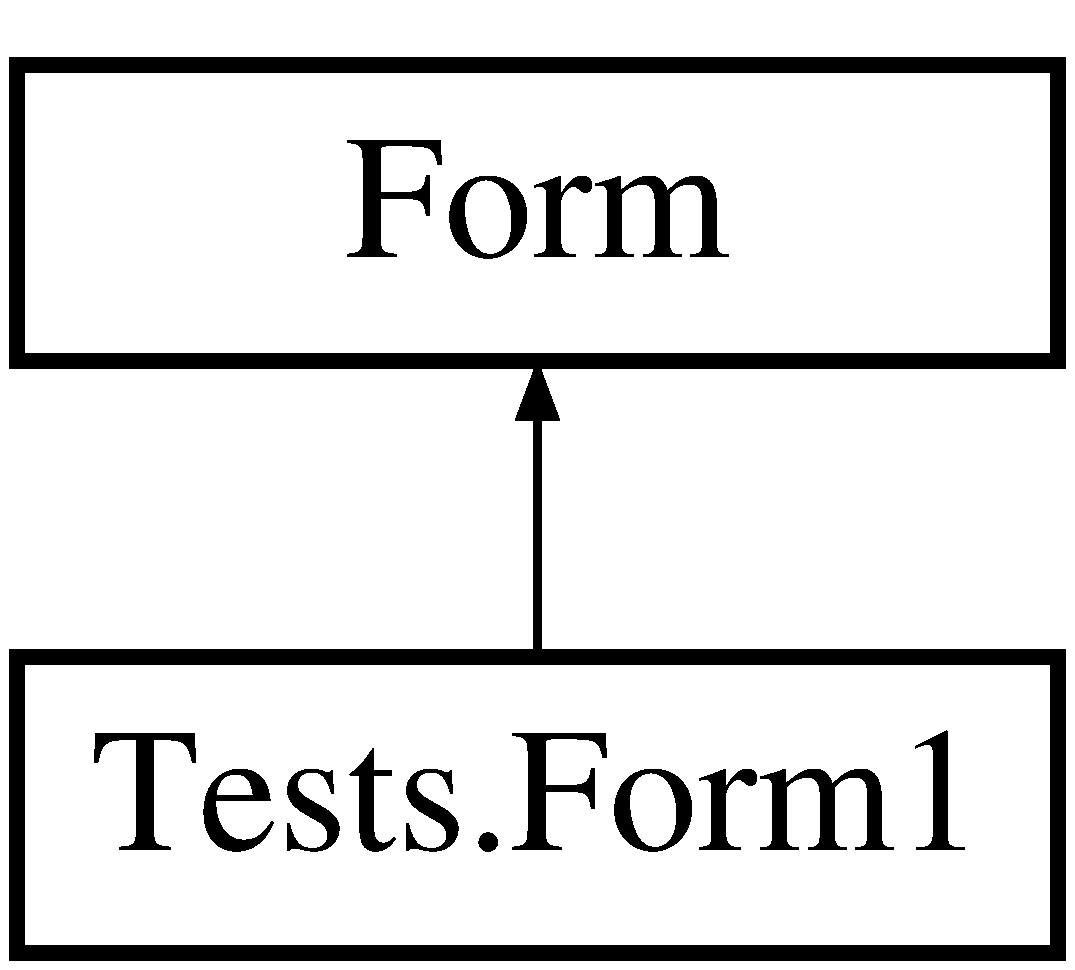
\includegraphics[height=2.000000cm]{class_tests_1_1_form1}
\end{center}
\end{figure}
\subsection*{Загальнодоступні елементи}
\begin{DoxyCompactItemize}
\item 
\hyperlink{class_tests_1_1_form1_a9a2a3898ba3628d71cd612c38887b85f}{Form1} ()
\begin{DoxyCompactList}\small\item\em констуркор першої форми \end{DoxyCompactList}\end{DoxyCompactItemize}
\subsection*{Захищені елементи}
\begin{DoxyCompactItemize}
\item 
override void \hyperlink{class_tests_1_1_form1_ad6c795827113080b827ff5bfd3267f38}{Dispose} (bool disposing)
\begin{DoxyCompactList}\small\item\em Clean up any resources being used. \end{DoxyCompactList}\end{DoxyCompactItemize}
\subsection*{Приватні елементи}
\begin{DoxyCompactItemize}
\item 
void \hyperlink{class_tests_1_1_form1_a861240fc111a9f0c68cdc64138e1a8e3}{button\+\_\+\+Sign\+In\+\_\+\+Click} (object sender, Event\+Args e)
\begin{DoxyCompactList}\small\item\em короткий опис детальний опис \end{DoxyCompactList}\item 
void \hyperlink{class_tests_1_1_form1_a607e53e1c4cb0f90ec5920fa5225f6bb}{button\+\_\+\+Registration\+\_\+\+Click} (object sender, Event\+Args e)
\item 
void \hyperlink{class_tests_1_1_form1_a66bdf3e4f89c528e5c2d6b1539db6488}{Initialize\+Component} ()
\begin{DoxyCompactList}\small\item\em Required method for Designer support -\/ do not modify the contents of this method with the code editor. \end{DoxyCompactList}\end{DoxyCompactItemize}
\subsection*{Приватні дані}
\begin{DoxyCompactItemize}
\item 
string \hyperlink{class_tests_1_1_form1_a5184480c920c20fa37adce88de490bd6}{read\+Text}
\item 
string \hyperlink{class_tests_1_1_form1_a4ed428771494f356b00fc2066168d3f8}{path} = @\char`\"{}tests\+File\textbackslash{}\+B\+D\+\_\+\+Login\+\_\+\+Password.\+txt\char`\"{}
\item 
System.\+Component\+Model.\+I\+Container \hyperlink{class_tests_1_1_form1_a98b604da06333c2647452a13c82d1266}{components} = null
\begin{DoxyCompactList}\small\item\em Required designer variable. \end{DoxyCompactList}\item 
System.\+Windows.\+Forms.\+Button \hyperlink{class_tests_1_1_form1_a8f99b3e333247f974869a05779c50c3b}{button\+\_\+\+Sign\+In}
\item 
System.\+Windows.\+Forms.\+Button \hyperlink{class_tests_1_1_form1_a0560759b788cb2777015e1d4fe1cf7cb}{button\+\_\+\+Registration}
\item 
System.\+Windows.\+Forms.\+Text\+Box \hyperlink{class_tests_1_1_form1_ac36a69acb7a9ed3387b08fd878c5f3ad}{text\+Box1}
\item 
System.\+Windows.\+Forms.\+Text\+Box \hyperlink{class_tests_1_1_form1_aa2d3b42202675e420de232a5bda1b156}{text\+Box2}
\item 
System.\+Windows.\+Forms.\+Label \hyperlink{class_tests_1_1_form1_acfe16ee506f1ce1e06fbe474a9ddc5b6}{label1}
\item 
System.\+Windows.\+Forms.\+Label \hyperlink{class_tests_1_1_form1_a83300d890a80130ed98355d16b01c06b}{label2}
\item 
System.\+Windows.\+Forms.\+Check\+Box \hyperlink{class_tests_1_1_form1_ad0eea4d9c6a082c8010281c105cc5a0e}{check\+Box\+\_\+adminka}
\end{DoxyCompactItemize}


\subsection{Конструктор(и)}
\index{Tests\+::\+Form1@{Tests\+::\+Form1}!Form1@{Form1}}
\index{Form1@{Form1}!Tests\+::\+Form1@{Tests\+::\+Form1}}
\subsubsection[{\texorpdfstring{Form1()}{Form1()}}]{\setlength{\rightskip}{0pt plus 5cm}Tests.\+Form1.\+Form1 (
\begin{DoxyParamCaption}
{}
\end{DoxyParamCaption}
)}\hypertarget{class_tests_1_1_form1_a9a2a3898ba3628d71cd612c38887b85f}{}\label{class_tests_1_1_form1_a9a2a3898ba3628d71cd612c38887b85f}


констуркор першої форми 

ініціалізує компоненти 

\subsection{Опис методів компонент}
\index{Tests\+::\+Form1@{Tests\+::\+Form1}!button\+\_\+\+Registration\+\_\+\+Click@{button\+\_\+\+Registration\+\_\+\+Click}}
\index{button\+\_\+\+Registration\+\_\+\+Click@{button\+\_\+\+Registration\+\_\+\+Click}!Tests\+::\+Form1@{Tests\+::\+Form1}}
\subsubsection[{\texorpdfstring{button\+\_\+\+Registration\+\_\+\+Click(object sender, Event\+Args e)}{button_Registration_Click(object sender, EventArgs e)}}]{\setlength{\rightskip}{0pt plus 5cm}void Tests.\+Form1.\+button\+\_\+\+Registration\+\_\+\+Click (
\begin{DoxyParamCaption}
\item[{object}]{sender, }
\item[{Event\+Args}]{e}
\end{DoxyParamCaption}
)\hspace{0.3cm}{\ttfamily [private]}}\hypertarget{class_tests_1_1_form1_a607e53e1c4cb0f90ec5920fa5225f6bb}{}\label{class_tests_1_1_form1_a607e53e1c4cb0f90ec5920fa5225f6bb}
\index{Tests\+::\+Form1@{Tests\+::\+Form1}!button\+\_\+\+Sign\+In\+\_\+\+Click@{button\+\_\+\+Sign\+In\+\_\+\+Click}}
\index{button\+\_\+\+Sign\+In\+\_\+\+Click@{button\+\_\+\+Sign\+In\+\_\+\+Click}!Tests\+::\+Form1@{Tests\+::\+Form1}}
\subsubsection[{\texorpdfstring{button\+\_\+\+Sign\+In\+\_\+\+Click(object sender, Event\+Args e)}{button_SignIn_Click(object sender, EventArgs e)}}]{\setlength{\rightskip}{0pt plus 5cm}void Tests.\+Form1.\+button\+\_\+\+Sign\+In\+\_\+\+Click (
\begin{DoxyParamCaption}
\item[{object}]{sender, }
\item[{Event\+Args}]{e}
\end{DoxyParamCaption}
)\hspace{0.3cm}{\ttfamily [private]}}\hypertarget{class_tests_1_1_form1_a861240fc111a9f0c68cdc64138e1a8e3}{}\label{class_tests_1_1_form1_a861240fc111a9f0c68cdc64138e1a8e3}


короткий опис детальний опис 

\begin{DoxyAuthor}{Автор}
maks 
\end{DoxyAuthor}
\begin{DoxyVersion}{Версія}
1.\+3 
\end{DoxyVersion}
\begin{DoxyRefDesc}{Необхідно зробити}
\item[\hyperlink{todo__todo000001}{Необхідно зробити}]something \end{DoxyRefDesc}

\begin{DoxyParams}{Аргументи}
{\em sender} & gggg \\
\hline
\end{DoxyParams}
\begin{DoxyReturn}{Повертає}
void 
\end{DoxyReturn}

\begin{DoxyExceptions}{Обробка виняткових ситуацій}
{\em Stack\+Overflow} & опис тут \\
\hline
\end{DoxyExceptions}
string t$<$ все що записано в текстовому \index{Tests\+::\+Form1@{Tests\+::\+Form1}!Dispose@{Dispose}}
\index{Dispose@{Dispose}!Tests\+::\+Form1@{Tests\+::\+Form1}}
\subsubsection[{\texorpdfstring{Dispose(bool disposing)}{Dispose(bool disposing)}}]{\setlength{\rightskip}{0pt plus 5cm}override void Tests.\+Form1.\+Dispose (
\begin{DoxyParamCaption}
\item[{bool}]{disposing}
\end{DoxyParamCaption}
)\hspace{0.3cm}{\ttfamily [protected]}}\hypertarget{class_tests_1_1_form1_ad6c795827113080b827ff5bfd3267f38}{}\label{class_tests_1_1_form1_ad6c795827113080b827ff5bfd3267f38}


Clean up any resources being used. 


\begin{DoxyParams}{Аргументи}
{\em disposing} & true if managed resources should be disposed; otherwise, false.\\
\hline
\end{DoxyParams}
\index{Tests\+::\+Form1@{Tests\+::\+Form1}!Initialize\+Component@{Initialize\+Component}}
\index{Initialize\+Component@{Initialize\+Component}!Tests\+::\+Form1@{Tests\+::\+Form1}}
\subsubsection[{\texorpdfstring{Initialize\+Component()}{InitializeComponent()}}]{\setlength{\rightskip}{0pt plus 5cm}void Tests.\+Form1.\+Initialize\+Component (
\begin{DoxyParamCaption}
{}
\end{DoxyParamCaption}
)\hspace{0.3cm}{\ttfamily [private]}}\hypertarget{class_tests_1_1_form1_a66bdf3e4f89c528e5c2d6b1539db6488}{}\label{class_tests_1_1_form1_a66bdf3e4f89c528e5c2d6b1539db6488}


Required method for Designer support -\/ do not modify the contents of this method with the code editor. 



\subsection{Компонентні дані}
\index{Tests\+::\+Form1@{Tests\+::\+Form1}!button\+\_\+\+Registration@{button\+\_\+\+Registration}}
\index{button\+\_\+\+Registration@{button\+\_\+\+Registration}!Tests\+::\+Form1@{Tests\+::\+Form1}}
\subsubsection[{\texorpdfstring{button\+\_\+\+Registration}{button_Registration}}]{\setlength{\rightskip}{0pt plus 5cm}System.\+Windows.\+Forms.\+Button Tests.\+Form1.\+button\+\_\+\+Registration\hspace{0.3cm}{\ttfamily [private]}}\hypertarget{class_tests_1_1_form1_a0560759b788cb2777015e1d4fe1cf7cb}{}\label{class_tests_1_1_form1_a0560759b788cb2777015e1d4fe1cf7cb}
\index{Tests\+::\+Form1@{Tests\+::\+Form1}!button\+\_\+\+Sign\+In@{button\+\_\+\+Sign\+In}}
\index{button\+\_\+\+Sign\+In@{button\+\_\+\+Sign\+In}!Tests\+::\+Form1@{Tests\+::\+Form1}}
\subsubsection[{\texorpdfstring{button\+\_\+\+Sign\+In}{button_SignIn}}]{\setlength{\rightskip}{0pt plus 5cm}System.\+Windows.\+Forms.\+Button Tests.\+Form1.\+button\+\_\+\+Sign\+In\hspace{0.3cm}{\ttfamily [private]}}\hypertarget{class_tests_1_1_form1_a8f99b3e333247f974869a05779c50c3b}{}\label{class_tests_1_1_form1_a8f99b3e333247f974869a05779c50c3b}
\index{Tests\+::\+Form1@{Tests\+::\+Form1}!check\+Box\+\_\+adminka@{check\+Box\+\_\+adminka}}
\index{check\+Box\+\_\+adminka@{check\+Box\+\_\+adminka}!Tests\+::\+Form1@{Tests\+::\+Form1}}
\subsubsection[{\texorpdfstring{check\+Box\+\_\+adminka}{checkBox_adminka}}]{\setlength{\rightskip}{0pt plus 5cm}System.\+Windows.\+Forms.\+Check\+Box Tests.\+Form1.\+check\+Box\+\_\+adminka\hspace{0.3cm}{\ttfamily [private]}}\hypertarget{class_tests_1_1_form1_ad0eea4d9c6a082c8010281c105cc5a0e}{}\label{class_tests_1_1_form1_ad0eea4d9c6a082c8010281c105cc5a0e}
\index{Tests\+::\+Form1@{Tests\+::\+Form1}!components@{components}}
\index{components@{components}!Tests\+::\+Form1@{Tests\+::\+Form1}}
\subsubsection[{\texorpdfstring{components}{components}}]{\setlength{\rightskip}{0pt plus 5cm}System.\+Component\+Model.\+I\+Container Tests.\+Form1.\+components = null\hspace{0.3cm}{\ttfamily [private]}}\hypertarget{class_tests_1_1_form1_a98b604da06333c2647452a13c82d1266}{}\label{class_tests_1_1_form1_a98b604da06333c2647452a13c82d1266}


Required designer variable. 

\index{Tests\+::\+Form1@{Tests\+::\+Form1}!label1@{label1}}
\index{label1@{label1}!Tests\+::\+Form1@{Tests\+::\+Form1}}
\subsubsection[{\texorpdfstring{label1}{label1}}]{\setlength{\rightskip}{0pt plus 5cm}System.\+Windows.\+Forms.\+Label Tests.\+Form1.\+label1\hspace{0.3cm}{\ttfamily [private]}}\hypertarget{class_tests_1_1_form1_acfe16ee506f1ce1e06fbe474a9ddc5b6}{}\label{class_tests_1_1_form1_acfe16ee506f1ce1e06fbe474a9ddc5b6}
\index{Tests\+::\+Form1@{Tests\+::\+Form1}!label2@{label2}}
\index{label2@{label2}!Tests\+::\+Form1@{Tests\+::\+Form1}}
\subsubsection[{\texorpdfstring{label2}{label2}}]{\setlength{\rightskip}{0pt plus 5cm}System.\+Windows.\+Forms.\+Label Tests.\+Form1.\+label2\hspace{0.3cm}{\ttfamily [private]}}\hypertarget{class_tests_1_1_form1_a83300d890a80130ed98355d16b01c06b}{}\label{class_tests_1_1_form1_a83300d890a80130ed98355d16b01c06b}
\index{Tests\+::\+Form1@{Tests\+::\+Form1}!path@{path}}
\index{path@{path}!Tests\+::\+Form1@{Tests\+::\+Form1}}
\subsubsection[{\texorpdfstring{path}{path}}]{\setlength{\rightskip}{0pt plus 5cm}string Tests.\+Form1.\+path = @\char`\"{}tests\+File\textbackslash{}\+B\+D\+\_\+\+Login\+\_\+\+Password.\+txt\char`\"{}\hspace{0.3cm}{\ttfamily [private]}}\hypertarget{class_tests_1_1_form1_a4ed428771494f356b00fc2066168d3f8}{}\label{class_tests_1_1_form1_a4ed428771494f356b00fc2066168d3f8}
\index{Tests\+::\+Form1@{Tests\+::\+Form1}!read\+Text@{read\+Text}}
\index{read\+Text@{read\+Text}!Tests\+::\+Form1@{Tests\+::\+Form1}}
\subsubsection[{\texorpdfstring{read\+Text}{readText}}]{\setlength{\rightskip}{0pt plus 5cm}string Tests.\+Form1.\+read\+Text\hspace{0.3cm}{\ttfamily [private]}}\hypertarget{class_tests_1_1_form1_a5184480c920c20fa37adce88de490bd6}{}\label{class_tests_1_1_form1_a5184480c920c20fa37adce88de490bd6}
\index{Tests\+::\+Form1@{Tests\+::\+Form1}!text\+Box1@{text\+Box1}}
\index{text\+Box1@{text\+Box1}!Tests\+::\+Form1@{Tests\+::\+Form1}}
\subsubsection[{\texorpdfstring{text\+Box1}{textBox1}}]{\setlength{\rightskip}{0pt plus 5cm}System.\+Windows.\+Forms.\+Text\+Box Tests.\+Form1.\+text\+Box1\hspace{0.3cm}{\ttfamily [private]}}\hypertarget{class_tests_1_1_form1_ac36a69acb7a9ed3387b08fd878c5f3ad}{}\label{class_tests_1_1_form1_ac36a69acb7a9ed3387b08fd878c5f3ad}
\index{Tests\+::\+Form1@{Tests\+::\+Form1}!text\+Box2@{text\+Box2}}
\index{text\+Box2@{text\+Box2}!Tests\+::\+Form1@{Tests\+::\+Form1}}
\subsubsection[{\texorpdfstring{text\+Box2}{textBox2}}]{\setlength{\rightskip}{0pt plus 5cm}System.\+Windows.\+Forms.\+Text\+Box Tests.\+Form1.\+text\+Box2\hspace{0.3cm}{\ttfamily [private]}}\hypertarget{class_tests_1_1_form1_aa2d3b42202675e420de232a5bda1b156}{}\label{class_tests_1_1_form1_aa2d3b42202675e420de232a5bda1b156}


Документація цих класів була створена з файлів\+:\begin{DoxyCompactItemize}
\item 
\hyperlink{_form1_8cs}{Form1.\+cs}\item 
\hyperlink{_form1_8_designer_8cs}{Form1.\+Designer.\+cs}\end{DoxyCompactItemize}

\hypertarget{class_tests_1_1_form2}{}\section{Клас Tests.\+Form2}
\label{class_tests_1_1_form2}\index{Tests.\+Form2@{Tests.\+Form2}}
Схема успадкувань для Tests.\+Form2\begin{figure}[H]
\begin{center}
\leavevmode
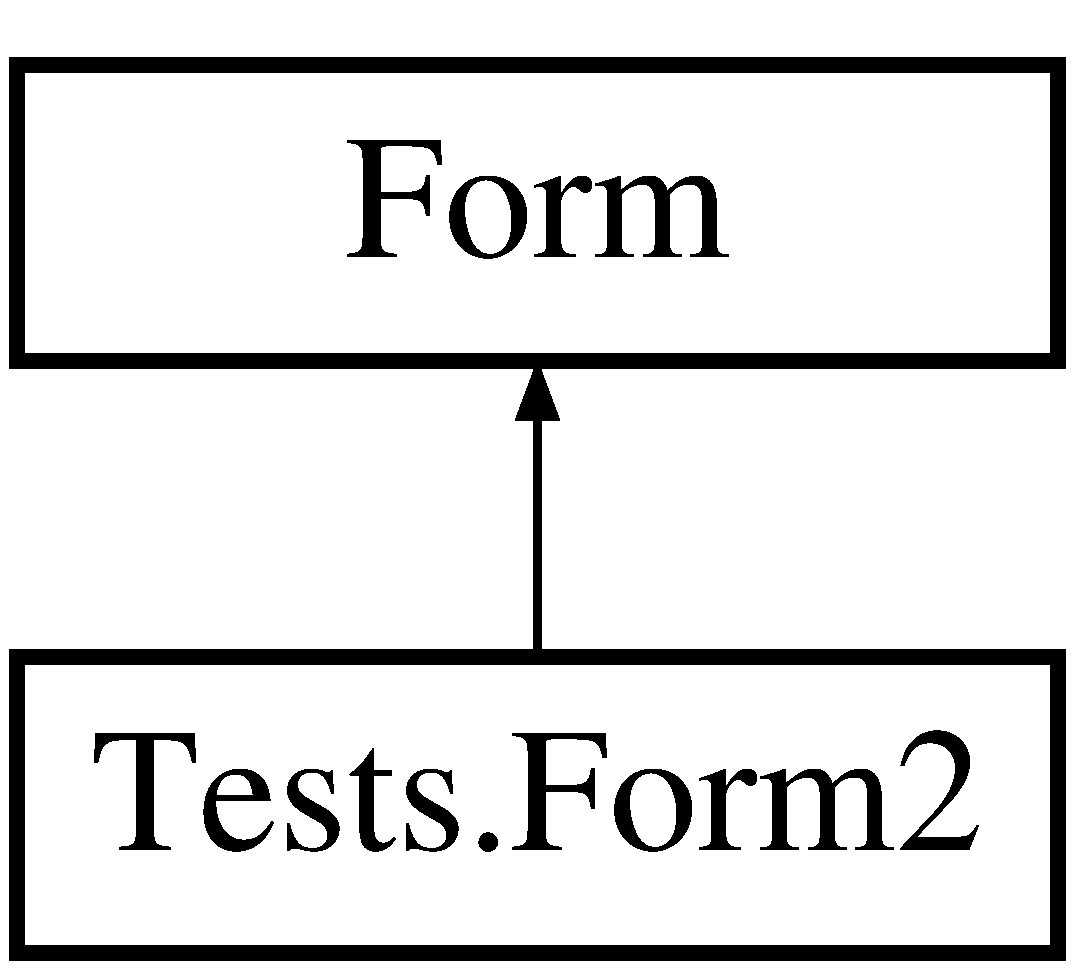
\includegraphics[height=2.000000cm]{class_tests_1_1_form2}
\end{center}
\end{figure}
\subsection*{Загальнодоступні елементи}
\begin{DoxyCompactItemize}
\item 
\hyperlink{class_tests_1_1_form2_a7e39b93c958b8e506e2d4da276f89e4d}{Form2} (string login)
\item 
void \hyperlink{class_tests_1_1_form2_af571b5761eaae8749d8c0fa64394dbc0}{History} (string User, string Question, string Choose\+Answer, bool is\+Correct)
\item 
void \hyperlink{class_tests_1_1_form2_af44e8c4f06da0c032f679825743fba6a}{Statistics} (string Login, int Count\+Mark, int Count\+Corect\+Mark)
\end{DoxyCompactItemize}
\subsection*{Захищені елементи}
\begin{DoxyCompactItemize}
\item 
override void \hyperlink{class_tests_1_1_form2_a8213f04aa4b31d28ee9f1a0f8842fb29}{Dispose} (bool disposing)
\begin{DoxyCompactList}\small\item\em Clean up any resources being used. \end{DoxyCompactList}\end{DoxyCompactItemize}
\subsection*{Приватні елементи}
\begin{DoxyCompactItemize}
\item 
void \hyperlink{class_tests_1_1_form2_a6290a2a05345f3a6220f589a3f52f3fa}{combo\+Box1\+\_\+\+Selected\+Index\+Changed} (object sender, Event\+Args e)
\item 
void \hyperlink{class_tests_1_1_form2_af46cfa9c6945e9e5b25b0e0face3ba4d}{button1\+\_\+\+Click} (object sender, Event\+Args e)
\item 
void \hyperlink{class_tests_1_1_form2_a3d7513211542e9311844b6641eb9fd61}{add\+Question} ()
\item 
void \hyperlink{class_tests_1_1_form2_ac597a8f0343f236b4d1ea528528e138c}{Initialize\+Component} ()
\begin{DoxyCompactList}\small\item\em Required method for Designer support -\/ do not modify the contents of this method with the code editor. \end{DoxyCompactList}\end{DoxyCompactItemize}
\subsection*{Приватні дані}
\begin{DoxyCompactItemize}
\item 
string \hyperlink{class_tests_1_1_form2_a94345348b49022de721b18d56a6ee69c}{user\+Name}
\item 
bool \hyperlink{class_tests_1_1_form2_a54e155db1ad24014b42f57316c451c8e}{Check\+History} = false
\item 
bool \hyperlink{class_tests_1_1_form2_a3757cb2e88f63fcddc6eafa8875d8083}{Check\+History2} = false
\item 
string\mbox{[}$\,$\mbox{]} \hyperlink{class_tests_1_1_form2_aac5d2866823577cccc4ca0a8442d2482}{str} = null
\item 
int \hyperlink{class_tests_1_1_form2_ad5c917043831c5e2e149a3f4c97c6bec}{i} = 0
\item 
int \hyperlink{class_tests_1_1_form2_a02950f1d6c4e43ab053c7b7aaeea873c}{str\+\_\+length} = 0
\item 
int \hyperlink{class_tests_1_1_form2_aa3d211b0601b3563a317d4af624ad95a}{good\+Answer} = 0
\item 
int \hyperlink{class_tests_1_1_form2_aa39ae1a993f54362add54ef965ceeb3d}{count\+Question} = 0
\item 
int \hyperlink{class_tests_1_1_form2_aa30b67a81604acf594bc26419d249f6f}{count\+Active} = 0
\item 
System.\+Component\+Model.\+I\+Container \hyperlink{class_tests_1_1_form2_a7d07edf4796d9dc60c94c70eefc79d72}{components} = null
\begin{DoxyCompactList}\small\item\em Required designer variable. \end{DoxyCompactList}\item 
System.\+Windows.\+Forms.\+Radio\+Button \hyperlink{class_tests_1_1_form2_aab1e99a28aeebaacbd56f13e46f7e276}{radio\+Button3}
\item 
System.\+Windows.\+Forms.\+Radio\+Button \hyperlink{class_tests_1_1_form2_a78bbfea2be8bda139a2ee7238c022d9a}{radio\+Button2}
\item 
System.\+Windows.\+Forms.\+Radio\+Button \hyperlink{class_tests_1_1_form2_ad4990affbee8ba8accb2b5aee47fdbca}{radio\+Button1}
\item 
System.\+Windows.\+Forms.\+Label \hyperlink{class_tests_1_1_form2_ad3b2b91e0f3feba4590909a3a7a183b6}{label1}
\item 
System.\+Windows.\+Forms.\+Button \hyperlink{class_tests_1_1_form2_a714a5d57a04e1dabbf37e3ab50da4050}{button\+\_\+ok}
\item 
System.\+Windows.\+Forms.\+List\+Box \hyperlink{class_tests_1_1_form2_a480f63340ce06b249c91e40b327e4ccb}{list\+Box1}
\item 
System.\+Windows.\+Forms.\+Combo\+Box \hyperlink{class_tests_1_1_form2_a2f3916e9df23010161dc15f6d047abae}{combo\+Box1}
\item 
System.\+Windows.\+Forms.\+Label \hyperlink{class_tests_1_1_form2_a8b4c39a636e8f658d2863be6160fc0ec}{label\+\_\+result}
\end{DoxyCompactItemize}


\subsection{Конструктор(и)}
\index{Tests\+::\+Form2@{Tests\+::\+Form2}!Form2@{Form2}}
\index{Form2@{Form2}!Tests\+::\+Form2@{Tests\+::\+Form2}}
\subsubsection[{\texorpdfstring{Form2(string login)}{Form2(string login)}}]{\setlength{\rightskip}{0pt plus 5cm}Tests.\+Form2.\+Form2 (
\begin{DoxyParamCaption}
\item[{string}]{login}
\end{DoxyParamCaption}
)}\hypertarget{class_tests_1_1_form2_a7e39b93c958b8e506e2d4da276f89e4d}{}\label{class_tests_1_1_form2_a7e39b93c958b8e506e2d4da276f89e4d}


\subsection{Опис методів компонент}
\index{Tests\+::\+Form2@{Tests\+::\+Form2}!add\+Question@{add\+Question}}
\index{add\+Question@{add\+Question}!Tests\+::\+Form2@{Tests\+::\+Form2}}
\subsubsection[{\texorpdfstring{add\+Question()}{addQuestion()}}]{\setlength{\rightskip}{0pt plus 5cm}void Tests.\+Form2.\+add\+Question (
\begin{DoxyParamCaption}
{}
\end{DoxyParamCaption}
)\hspace{0.3cm}{\ttfamily [private]}}\hypertarget{class_tests_1_1_form2_a3d7513211542e9311844b6641eb9fd61}{}\label{class_tests_1_1_form2_a3d7513211542e9311844b6641eb9fd61}
\index{Tests\+::\+Form2@{Tests\+::\+Form2}!button1\+\_\+\+Click@{button1\+\_\+\+Click}}
\index{button1\+\_\+\+Click@{button1\+\_\+\+Click}!Tests\+::\+Form2@{Tests\+::\+Form2}}
\subsubsection[{\texorpdfstring{button1\+\_\+\+Click(object sender, Event\+Args e)}{button1_Click(object sender, EventArgs e)}}]{\setlength{\rightskip}{0pt plus 5cm}void Tests.\+Form2.\+button1\+\_\+\+Click (
\begin{DoxyParamCaption}
\item[{object}]{sender, }
\item[{Event\+Args}]{e}
\end{DoxyParamCaption}
)\hspace{0.3cm}{\ttfamily [private]}}\hypertarget{class_tests_1_1_form2_af46cfa9c6945e9e5b25b0e0face3ba4d}{}\label{class_tests_1_1_form2_af46cfa9c6945e9e5b25b0e0face3ba4d}
\index{Tests\+::\+Form2@{Tests\+::\+Form2}!combo\+Box1\+\_\+\+Selected\+Index\+Changed@{combo\+Box1\+\_\+\+Selected\+Index\+Changed}}
\index{combo\+Box1\+\_\+\+Selected\+Index\+Changed@{combo\+Box1\+\_\+\+Selected\+Index\+Changed}!Tests\+::\+Form2@{Tests\+::\+Form2}}
\subsubsection[{\texorpdfstring{combo\+Box1\+\_\+\+Selected\+Index\+Changed(object sender, Event\+Args e)}{comboBox1_SelectedIndexChanged(object sender, EventArgs e)}}]{\setlength{\rightskip}{0pt plus 5cm}void Tests.\+Form2.\+combo\+Box1\+\_\+\+Selected\+Index\+Changed (
\begin{DoxyParamCaption}
\item[{object}]{sender, }
\item[{Event\+Args}]{e}
\end{DoxyParamCaption}
)\hspace{0.3cm}{\ttfamily [private]}}\hypertarget{class_tests_1_1_form2_a6290a2a05345f3a6220f589a3f52f3fa}{}\label{class_tests_1_1_form2_a6290a2a05345f3a6220f589a3f52f3fa}
\index{Tests\+::\+Form2@{Tests\+::\+Form2}!Dispose@{Dispose}}
\index{Dispose@{Dispose}!Tests\+::\+Form2@{Tests\+::\+Form2}}
\subsubsection[{\texorpdfstring{Dispose(bool disposing)}{Dispose(bool disposing)}}]{\setlength{\rightskip}{0pt plus 5cm}override void Tests.\+Form2.\+Dispose (
\begin{DoxyParamCaption}
\item[{bool}]{disposing}
\end{DoxyParamCaption}
)\hspace{0.3cm}{\ttfamily [protected]}}\hypertarget{class_tests_1_1_form2_a8213f04aa4b31d28ee9f1a0f8842fb29}{}\label{class_tests_1_1_form2_a8213f04aa4b31d28ee9f1a0f8842fb29}


Clean up any resources being used. 


\begin{DoxyParams}{Аргументи}
{\em disposing} & true if managed resources should be disposed; otherwise, false.\\
\hline
\end{DoxyParams}
\index{Tests\+::\+Form2@{Tests\+::\+Form2}!History@{History}}
\index{History@{History}!Tests\+::\+Form2@{Tests\+::\+Form2}}
\subsubsection[{\texorpdfstring{History(string User, string Question, string Choose\+Answer, bool is\+Correct)}{History(string User, string Question, string ChooseAnswer, bool isCorrect)}}]{\setlength{\rightskip}{0pt plus 5cm}void Tests.\+Form2.\+History (
\begin{DoxyParamCaption}
\item[{string}]{User, }
\item[{string}]{Question, }
\item[{string}]{Choose\+Answer, }
\item[{bool}]{is\+Correct}
\end{DoxyParamCaption}
)}\hypertarget{class_tests_1_1_form2_af571b5761eaae8749d8c0fa64394dbc0}{}\label{class_tests_1_1_form2_af571b5761eaae8749d8c0fa64394dbc0}
\index{Tests\+::\+Form2@{Tests\+::\+Form2}!Initialize\+Component@{Initialize\+Component}}
\index{Initialize\+Component@{Initialize\+Component}!Tests\+::\+Form2@{Tests\+::\+Form2}}
\subsubsection[{\texorpdfstring{Initialize\+Component()}{InitializeComponent()}}]{\setlength{\rightskip}{0pt plus 5cm}void Tests.\+Form2.\+Initialize\+Component (
\begin{DoxyParamCaption}
{}
\end{DoxyParamCaption}
)\hspace{0.3cm}{\ttfamily [private]}}\hypertarget{class_tests_1_1_form2_ac597a8f0343f236b4d1ea528528e138c}{}\label{class_tests_1_1_form2_ac597a8f0343f236b4d1ea528528e138c}


Required method for Designer support -\/ do not modify the contents of this method with the code editor. 

\index{Tests\+::\+Form2@{Tests\+::\+Form2}!Statistics@{Statistics}}
\index{Statistics@{Statistics}!Tests\+::\+Form2@{Tests\+::\+Form2}}
\subsubsection[{\texorpdfstring{Statistics(string Login, int Count\+Mark, int Count\+Corect\+Mark)}{Statistics(string Login, int CountMark, int CountCorectMark)}}]{\setlength{\rightskip}{0pt plus 5cm}void Tests.\+Form2.\+Statistics (
\begin{DoxyParamCaption}
\item[{string}]{Login, }
\item[{int}]{Count\+Mark, }
\item[{int}]{Count\+Corect\+Mark}
\end{DoxyParamCaption}
)}\hypertarget{class_tests_1_1_form2_af44e8c4f06da0c032f679825743fba6a}{}\label{class_tests_1_1_form2_af44e8c4f06da0c032f679825743fba6a}


\subsection{Компонентні дані}
\index{Tests\+::\+Form2@{Tests\+::\+Form2}!button\+\_\+ok@{button\+\_\+ok}}
\index{button\+\_\+ok@{button\+\_\+ok}!Tests\+::\+Form2@{Tests\+::\+Form2}}
\subsubsection[{\texorpdfstring{button\+\_\+ok}{button_ok}}]{\setlength{\rightskip}{0pt plus 5cm}System.\+Windows.\+Forms.\+Button Tests.\+Form2.\+button\+\_\+ok\hspace{0.3cm}{\ttfamily [private]}}\hypertarget{class_tests_1_1_form2_a714a5d57a04e1dabbf37e3ab50da4050}{}\label{class_tests_1_1_form2_a714a5d57a04e1dabbf37e3ab50da4050}
\index{Tests\+::\+Form2@{Tests\+::\+Form2}!Check\+History@{Check\+History}}
\index{Check\+History@{Check\+History}!Tests\+::\+Form2@{Tests\+::\+Form2}}
\subsubsection[{\texorpdfstring{Check\+History}{CheckHistory}}]{\setlength{\rightskip}{0pt plus 5cm}bool Tests.\+Form2.\+Check\+History = false\hspace{0.3cm}{\ttfamily [private]}}\hypertarget{class_tests_1_1_form2_a54e155db1ad24014b42f57316c451c8e}{}\label{class_tests_1_1_form2_a54e155db1ad24014b42f57316c451c8e}
\index{Tests\+::\+Form2@{Tests\+::\+Form2}!Check\+History2@{Check\+History2}}
\index{Check\+History2@{Check\+History2}!Tests\+::\+Form2@{Tests\+::\+Form2}}
\subsubsection[{\texorpdfstring{Check\+History2}{CheckHistory2}}]{\setlength{\rightskip}{0pt plus 5cm}bool Tests.\+Form2.\+Check\+History2 = false\hspace{0.3cm}{\ttfamily [private]}}\hypertarget{class_tests_1_1_form2_a3757cb2e88f63fcddc6eafa8875d8083}{}\label{class_tests_1_1_form2_a3757cb2e88f63fcddc6eafa8875d8083}
\index{Tests\+::\+Form2@{Tests\+::\+Form2}!combo\+Box1@{combo\+Box1}}
\index{combo\+Box1@{combo\+Box1}!Tests\+::\+Form2@{Tests\+::\+Form2}}
\subsubsection[{\texorpdfstring{combo\+Box1}{comboBox1}}]{\setlength{\rightskip}{0pt plus 5cm}System.\+Windows.\+Forms.\+Combo\+Box Tests.\+Form2.\+combo\+Box1\hspace{0.3cm}{\ttfamily [private]}}\hypertarget{class_tests_1_1_form2_a2f3916e9df23010161dc15f6d047abae}{}\label{class_tests_1_1_form2_a2f3916e9df23010161dc15f6d047abae}
\index{Tests\+::\+Form2@{Tests\+::\+Form2}!components@{components}}
\index{components@{components}!Tests\+::\+Form2@{Tests\+::\+Form2}}
\subsubsection[{\texorpdfstring{components}{components}}]{\setlength{\rightskip}{0pt plus 5cm}System.\+Component\+Model.\+I\+Container Tests.\+Form2.\+components = null\hspace{0.3cm}{\ttfamily [private]}}\hypertarget{class_tests_1_1_form2_a7d07edf4796d9dc60c94c70eefc79d72}{}\label{class_tests_1_1_form2_a7d07edf4796d9dc60c94c70eefc79d72}


Required designer variable. 

\index{Tests\+::\+Form2@{Tests\+::\+Form2}!count\+Active@{count\+Active}}
\index{count\+Active@{count\+Active}!Tests\+::\+Form2@{Tests\+::\+Form2}}
\subsubsection[{\texorpdfstring{count\+Active}{countActive}}]{\setlength{\rightskip}{0pt plus 5cm}int Tests.\+Form2.\+count\+Active = 0\hspace{0.3cm}{\ttfamily [private]}}\hypertarget{class_tests_1_1_form2_aa30b67a81604acf594bc26419d249f6f}{}\label{class_tests_1_1_form2_aa30b67a81604acf594bc26419d249f6f}
\index{Tests\+::\+Form2@{Tests\+::\+Form2}!count\+Question@{count\+Question}}
\index{count\+Question@{count\+Question}!Tests\+::\+Form2@{Tests\+::\+Form2}}
\subsubsection[{\texorpdfstring{count\+Question}{countQuestion}}]{\setlength{\rightskip}{0pt plus 5cm}int Tests.\+Form2.\+count\+Question = 0\hspace{0.3cm}{\ttfamily [private]}}\hypertarget{class_tests_1_1_form2_aa39ae1a993f54362add54ef965ceeb3d}{}\label{class_tests_1_1_form2_aa39ae1a993f54362add54ef965ceeb3d}
\index{Tests\+::\+Form2@{Tests\+::\+Form2}!good\+Answer@{good\+Answer}}
\index{good\+Answer@{good\+Answer}!Tests\+::\+Form2@{Tests\+::\+Form2}}
\subsubsection[{\texorpdfstring{good\+Answer}{goodAnswer}}]{\setlength{\rightskip}{0pt plus 5cm}int Tests.\+Form2.\+good\+Answer = 0\hspace{0.3cm}{\ttfamily [private]}}\hypertarget{class_tests_1_1_form2_aa3d211b0601b3563a317d4af624ad95a}{}\label{class_tests_1_1_form2_aa3d211b0601b3563a317d4af624ad95a}
\index{Tests\+::\+Form2@{Tests\+::\+Form2}!i@{i}}
\index{i@{i}!Tests\+::\+Form2@{Tests\+::\+Form2}}
\subsubsection[{\texorpdfstring{i}{i}}]{\setlength{\rightskip}{0pt plus 5cm}int Tests.\+Form2.\+i = 0\hspace{0.3cm}{\ttfamily [private]}}\hypertarget{class_tests_1_1_form2_ad5c917043831c5e2e149a3f4c97c6bec}{}\label{class_tests_1_1_form2_ad5c917043831c5e2e149a3f4c97c6bec}
\index{Tests\+::\+Form2@{Tests\+::\+Form2}!label1@{label1}}
\index{label1@{label1}!Tests\+::\+Form2@{Tests\+::\+Form2}}
\subsubsection[{\texorpdfstring{label1}{label1}}]{\setlength{\rightskip}{0pt plus 5cm}System.\+Windows.\+Forms.\+Label Tests.\+Form2.\+label1\hspace{0.3cm}{\ttfamily [private]}}\hypertarget{class_tests_1_1_form2_ad3b2b91e0f3feba4590909a3a7a183b6}{}\label{class_tests_1_1_form2_ad3b2b91e0f3feba4590909a3a7a183b6}
\index{Tests\+::\+Form2@{Tests\+::\+Form2}!label\+\_\+result@{label\+\_\+result}}
\index{label\+\_\+result@{label\+\_\+result}!Tests\+::\+Form2@{Tests\+::\+Form2}}
\subsubsection[{\texorpdfstring{label\+\_\+result}{label_result}}]{\setlength{\rightskip}{0pt plus 5cm}System.\+Windows.\+Forms.\+Label Tests.\+Form2.\+label\+\_\+result\hspace{0.3cm}{\ttfamily [private]}}\hypertarget{class_tests_1_1_form2_a8b4c39a636e8f658d2863be6160fc0ec}{}\label{class_tests_1_1_form2_a8b4c39a636e8f658d2863be6160fc0ec}
\index{Tests\+::\+Form2@{Tests\+::\+Form2}!list\+Box1@{list\+Box1}}
\index{list\+Box1@{list\+Box1}!Tests\+::\+Form2@{Tests\+::\+Form2}}
\subsubsection[{\texorpdfstring{list\+Box1}{listBox1}}]{\setlength{\rightskip}{0pt plus 5cm}System.\+Windows.\+Forms.\+List\+Box Tests.\+Form2.\+list\+Box1\hspace{0.3cm}{\ttfamily [private]}}\hypertarget{class_tests_1_1_form2_a480f63340ce06b249c91e40b327e4ccb}{}\label{class_tests_1_1_form2_a480f63340ce06b249c91e40b327e4ccb}
\index{Tests\+::\+Form2@{Tests\+::\+Form2}!radio\+Button1@{radio\+Button1}}
\index{radio\+Button1@{radio\+Button1}!Tests\+::\+Form2@{Tests\+::\+Form2}}
\subsubsection[{\texorpdfstring{radio\+Button1}{radioButton1}}]{\setlength{\rightskip}{0pt plus 5cm}System.\+Windows.\+Forms.\+Radio\+Button Tests.\+Form2.\+radio\+Button1\hspace{0.3cm}{\ttfamily [private]}}\hypertarget{class_tests_1_1_form2_ad4990affbee8ba8accb2b5aee47fdbca}{}\label{class_tests_1_1_form2_ad4990affbee8ba8accb2b5aee47fdbca}
\index{Tests\+::\+Form2@{Tests\+::\+Form2}!radio\+Button2@{radio\+Button2}}
\index{radio\+Button2@{radio\+Button2}!Tests\+::\+Form2@{Tests\+::\+Form2}}
\subsubsection[{\texorpdfstring{radio\+Button2}{radioButton2}}]{\setlength{\rightskip}{0pt plus 5cm}System.\+Windows.\+Forms.\+Radio\+Button Tests.\+Form2.\+radio\+Button2\hspace{0.3cm}{\ttfamily [private]}}\hypertarget{class_tests_1_1_form2_a78bbfea2be8bda139a2ee7238c022d9a}{}\label{class_tests_1_1_form2_a78bbfea2be8bda139a2ee7238c022d9a}
\index{Tests\+::\+Form2@{Tests\+::\+Form2}!radio\+Button3@{radio\+Button3}}
\index{radio\+Button3@{radio\+Button3}!Tests\+::\+Form2@{Tests\+::\+Form2}}
\subsubsection[{\texorpdfstring{radio\+Button3}{radioButton3}}]{\setlength{\rightskip}{0pt plus 5cm}System.\+Windows.\+Forms.\+Radio\+Button Tests.\+Form2.\+radio\+Button3\hspace{0.3cm}{\ttfamily [private]}}\hypertarget{class_tests_1_1_form2_aab1e99a28aeebaacbd56f13e46f7e276}{}\label{class_tests_1_1_form2_aab1e99a28aeebaacbd56f13e46f7e276}
\index{Tests\+::\+Form2@{Tests\+::\+Form2}!str@{str}}
\index{str@{str}!Tests\+::\+Form2@{Tests\+::\+Form2}}
\subsubsection[{\texorpdfstring{str}{str}}]{\setlength{\rightskip}{0pt plus 5cm}string \mbox{[}$\,$\mbox{]} Tests.\+Form2.\+str = null\hspace{0.3cm}{\ttfamily [private]}}\hypertarget{class_tests_1_1_form2_aac5d2866823577cccc4ca0a8442d2482}{}\label{class_tests_1_1_form2_aac5d2866823577cccc4ca0a8442d2482}
\index{Tests\+::\+Form2@{Tests\+::\+Form2}!str\+\_\+length@{str\+\_\+length}}
\index{str\+\_\+length@{str\+\_\+length}!Tests\+::\+Form2@{Tests\+::\+Form2}}
\subsubsection[{\texorpdfstring{str\+\_\+length}{str_length}}]{\setlength{\rightskip}{0pt plus 5cm}int Tests.\+Form2.\+str\+\_\+length = 0\hspace{0.3cm}{\ttfamily [private]}}\hypertarget{class_tests_1_1_form2_a02950f1d6c4e43ab053c7b7aaeea873c}{}\label{class_tests_1_1_form2_a02950f1d6c4e43ab053c7b7aaeea873c}
\index{Tests\+::\+Form2@{Tests\+::\+Form2}!user\+Name@{user\+Name}}
\index{user\+Name@{user\+Name}!Tests\+::\+Form2@{Tests\+::\+Form2}}
\subsubsection[{\texorpdfstring{user\+Name}{userName}}]{\setlength{\rightskip}{0pt plus 5cm}string Tests.\+Form2.\+user\+Name\hspace{0.3cm}{\ttfamily [private]}}\hypertarget{class_tests_1_1_form2_a94345348b49022de721b18d56a6ee69c}{}\label{class_tests_1_1_form2_a94345348b49022de721b18d56a6ee69c}


Документація цих класів була створена з файлів\+:\begin{DoxyCompactItemize}
\item 
\hyperlink{_form2_8cs}{Form2.\+cs}\item 
\hyperlink{_form2_8_designer_8cs}{Form2.\+Designer.\+cs}\end{DoxyCompactItemize}

\hypertarget{class_tests_1_1_program}{}\section{Клас Tests.\+Program}
\label{class_tests_1_1_program}\index{Tests.\+Program@{Tests.\+Program}}
\subsection*{Приватні статичні елементи}
\begin{DoxyCompactItemize}
\item 
static void \hyperlink{class_tests_1_1_program_ae3235f237d6510e0f706a7af7cbfe3c0}{Main} ()
\begin{DoxyCompactList}\small\item\em The main entry point for the application. \end{DoxyCompactList}\end{DoxyCompactItemize}


\subsection{Опис методів компонент}
\index{Tests\+::\+Program@{Tests\+::\+Program}!Main@{Main}}
\index{Main@{Main}!Tests\+::\+Program@{Tests\+::\+Program}}
\subsubsection[{\texorpdfstring{Main()}{Main()}}]{\setlength{\rightskip}{0pt plus 5cm}static void Tests.\+Program.\+Main (
\begin{DoxyParamCaption}
{}
\end{DoxyParamCaption}
)\hspace{0.3cm}{\ttfamily [static]}, {\ttfamily [private]}}\hypertarget{class_tests_1_1_program_ae3235f237d6510e0f706a7af7cbfe3c0}{}\label{class_tests_1_1_program_ae3235f237d6510e0f706a7af7cbfe3c0}


The main entry point for the application. 



Документація цього класу була створена з файлу\+:\begin{DoxyCompactItemize}
\item 
\hyperlink{_program_8cs}{Program.\+cs}\end{DoxyCompactItemize}

\chapter{Файли}
\hypertarget{_adminka_8cs}{}\section{Файл Adminka.\+cs}
\label{_adminka_8cs}\index{Adminka.\+cs@{Adminka.\+cs}}
\subsection*{Класи}
\begin{DoxyCompactItemize}
\item 
class \hyperlink{class_tests_1_1_adminka}{Tests.\+Adminka}
\end{DoxyCompactItemize}
\subsection*{Простори імен}
\begin{DoxyCompactItemize}
\item 
namespace \hyperlink{namespace_tests}{Tests}
\end{DoxyCompactItemize}

\hypertarget{_adminka_8_designer_8cs}{}\section{Файл Adminka.\+Designer.\+cs}
\label{_adminka_8_designer_8cs}\index{Adminka.\+Designer.\+cs@{Adminka.\+Designer.\+cs}}
\subsection*{Класи}
\begin{DoxyCompactItemize}
\item 
class \hyperlink{class_tests_1_1_adminka}{Tests.\+Adminka}
\end{DoxyCompactItemize}
\subsection*{Простори імен}
\begin{DoxyCompactItemize}
\item 
namespace \hyperlink{namespace_tests}{Tests}
\end{DoxyCompactItemize}

\hypertarget{_form1_8cs}{}\section{Файл Form1.\+cs}
\label{_form1_8cs}\index{Form1.\+cs@{Form1.\+cs}}
\subsection*{Класи}
\begin{DoxyCompactItemize}
\item 
class \hyperlink{class_tests_1_1_form1}{Tests.\+Form1}
\end{DoxyCompactItemize}
\subsection*{Простори імен}
\begin{DoxyCompactItemize}
\item 
namespace \hyperlink{namespace_tests}{Tests}
\end{DoxyCompactItemize}

\hypertarget{_form1_8_designer_8cs}{}\section{Файл Form1.\+Designer.\+cs}
\label{_form1_8_designer_8cs}\index{Form1.\+Designer.\+cs@{Form1.\+Designer.\+cs}}
\subsection*{Класи}
\begin{DoxyCompactItemize}
\item 
class \hyperlink{class_tests_1_1_form1}{Tests.\+Form1}
\end{DoxyCompactItemize}
\subsection*{Простори імен}
\begin{DoxyCompactItemize}
\item 
namespace \hyperlink{namespace_tests}{Tests}
\end{DoxyCompactItemize}

\hypertarget{_form2_8cs}{}\section{Файл Form2.\+cs}
\label{_form2_8cs}\index{Form2.\+cs@{Form2.\+cs}}
\subsection*{Класи}
\begin{DoxyCompactItemize}
\item 
class \hyperlink{class_tests_1_1_form2}{Tests.\+Form2}
\end{DoxyCompactItemize}
\subsection*{Простори імен}
\begin{DoxyCompactItemize}
\item 
namespace \hyperlink{namespace_tests}{Tests}
\end{DoxyCompactItemize}

\hypertarget{_form2_8_designer_8cs}{}\section{Файл Form2.\+Designer.\+cs}
\label{_form2_8_designer_8cs}\index{Form2.\+Designer.\+cs@{Form2.\+Designer.\+cs}}
\subsection*{Класи}
\begin{DoxyCompactItemize}
\item 
class \hyperlink{class_tests_1_1_form2}{Tests.\+Form2}
\end{DoxyCompactItemize}
\subsection*{Простори імен}
\begin{DoxyCompactItemize}
\item 
namespace \hyperlink{namespace_tests}{Tests}
\end{DoxyCompactItemize}

\hypertarget{_program_8cs}{}\section{Файл Program.\+cs}
\label{_program_8cs}\index{Program.\+cs@{Program.\+cs}}
\subsection*{Класи}
\begin{DoxyCompactItemize}
\item 
class \hyperlink{class_tests_1_1_program}{Tests.\+Program}
\end{DoxyCompactItemize}
\subsection*{Простори імен}
\begin{DoxyCompactItemize}
\item 
namespace \hyperlink{namespace_tests}{Tests}
\end{DoxyCompactItemize}

%--- End generated contents ---

% Index
\backmatter
\newpage
\phantomsection
\clearemptydoublepage
\addcontentsline{toc}{chapter}{Предметний покажчик}
\printindex

\end{document}
